\documentclass[a4paper]{book}
\usepackage{a4wide}
\usepackage{makeidx}
\usepackage{graphicx}
\usepackage{multicol}
\usepackage{float}
\usepackage{listings}
\usepackage{color}
\usepackage{textcomp}
\usepackage{alltt}
\usepackage{times}
\usepackage{ifpdf}
\ifpdf
\usepackage[pdftex,
            pagebackref=true,
            colorlinks=true,
            linkcolor=blue,
            unicode
           ]{hyperref}
\else
\usepackage[ps2pdf,
            pagebackref=true,
            colorlinks=true,
            linkcolor=blue,
            unicode
           ]{hyperref}
\usepackage{pspicture}
\fi
\usepackage[utf8]{inputenc}
\usepackage{doxygen}
\lstset{language=C++,inputencoding=utf8,basicstyle=\footnotesize,breaklines=true,breakatwhitespace=true,tabsize=8,numbers=left }
\makeindex
\setcounter{tocdepth}{3}
\renewcommand{\footrulewidth}{0.4pt}
\begin{document}
\hypersetup{pageanchor=false}
\begin{titlepage}
\vspace*{7cm}
\begin{center}
{\Large Qcorr: A Digital Image Correlation Program implemented in QT4 \\[1ex]\large 1.0 }\\
\vspace*{1cm}
{\large Generated by Doxygen 1.6.1}\\
\vspace*{0.5cm}
{\small Sun Dec 6 00:22:28 2009}\\
\end{center}
\end{titlepage}
\clearemptydoublepage
\pagenumbering{roman}
\tableofcontents
\clearemptydoublepage
\pagenumbering{arabic}
\hypersetup{pageanchor=true}
\chapter{Todo List}
\label{todo}
\hypertarget{todo}{}
\label{todo__todo000001}
\hypertarget{todo__todo000001}{}
 
\begin{DoxyDescription}
\item[Class \hyperlink{classQcorr}{Qcorr} ]
\begin{DoxyItemize}
\item Add Stereo functionality to obtain disparity maps
\end{DoxyItemize}


\end{DoxyDescription}
\chapter{Bug List}
\label{bug}
\hypertarget{bug}{}
\label{bug__bug000001}
\hypertarget{bug__bug000001}{}
 
\begin{DoxyDescription}
\item[Class \hyperlink{classQcorr}{Qcorr} ]
\begin{DoxyItemize}
\item Perhaps a few, but not noticed so far.
\end{DoxyItemize}


\end{DoxyDescription}
\chapter{Module Index}
\section{Modules}
Here is a list of all modules:\begin{CompactList}
\item \contentsline{section}{Qcorr}{\pageref{group__qcorr__mainwindow}}{}
\end{CompactList}

\chapter{Class Index}
\section{Class Hierarchy}
This inheritance list is sorted roughly, but not completely, alphabetically:\begin{DoxyCompactList}
\item \contentsline{section}{CorrMethod}{\pageref{classCorrMethod}}{}
\item \contentsline{section}{ImgLabel}{\pageref{classImgLabel}}{}
\item \contentsline{section}{TargetImgLabel}{\pageref{classTargetImgLabel}}{}
\item \contentsline{section}{Ui\_\-CorrMethodClass}{\pageref{classUi__CorrMethodClass}}{}
\begin{DoxyCompactList}
\item \contentsline{section}{Ui::CorrMethodClass}{\pageref{classUi_1_1CorrMethodClass}}{}
\end{DoxyCompactList}
\item \contentsline{section}{Ui\_\-QcorrClass}{\pageref{classUi__QcorrClass}}{}
\begin{DoxyCompactList}
\item \contentsline{section}{Ui::QcorrClass}{\pageref{classUi_1_1QcorrClass}}{}
\begin{DoxyCompactList}
\item \contentsline{section}{Qcorr}{\pageref{classQcorr}}{}
\end{DoxyCompactList}
\end{DoxyCompactList}
\end{DoxyCompactList}

\chapter{Class Index}
\section{Class List}
Here are the classes, structs, unions and interfaces with brief descriptions:\begin{CompactList}
\item\contentsline{section}{\hyperlink{classImgLabel}{ImgLabel} (\hyperlink{classImgLabel}{ImgLabel} class is a friend of \hyperlink{classQcorr}{Qcorr} in order to make all members of \hyperlink{classQcorr}{Qcorr} accessible by an \hyperlink{classImgLabel}{ImgLabel} object )}{\pageref{classImgLabel}}{}
\item\contentsline{section}{\hyperlink{classQcorr}{Qcorr} (A Digital Image Correlation Program (Template Matcher) implemented in QT4 )}{\pageref{classQcorr}}{}
\end{CompactList}

\chapter{Module Documentation}
\hypertarget{group__qcorr__mainwindow}{
\section{Qcorr}
\label{group__qcorr__mainwindow}\index{Qcorr@{Qcorr}}
}
\subsection*{Classes}
\begin{DoxyCompactItemize}
\item 
class \hyperlink{classQcorr}{Qcorr}
\begin{DoxyCompactList}\small\item\em friend of this \hyperlink{classImgLabel}{ImgLabel} class, so all members from \hyperlink{classImgLabel}{ImgLabel} are accessible by a \hyperlink{classQcorr}{Qcorr} object \item\end{DoxyCompactList}\end{DoxyCompactItemize}

\chapter{Class Documentation}
\input{classControlsWindow}
\include{classControlsWindow}
\include{classUi_1_1ControlsWindowClass}
\hypertarget{classCorrMethod}{
\section{CorrMethod Class Reference}
\label{classCorrMethod}\index{CorrMethod@{CorrMethod}}
}
\subsection*{Public Member Functions}
\begin{DoxyCompactItemize}
\item 
\hypertarget{classCorrMethod_abdc14398267291249d40158e133cf68b}{
{\bfseries CorrMethod} (QWidget $\ast$parent=0)}
\label{classCorrMethod_abdc14398267291249d40158e133cf68b}

\item 
int \hyperlink{classCorrMethod_a3eeafdd901560c1fa92be75d4ed58872}{getMethod} ()
\begin{DoxyCompactList}\small\item\em Retrieve the selected method to be used in the correlation process. \item\end{DoxyCompactList}\end{DoxyCompactItemize}
\subsection*{Private Slots}
\begin{DoxyCompactItemize}
\item 
\hypertarget{classCorrMethod_a87e628d7ef6facc9a402880d7e01ea36}{
void {\bfseries cancelMethod} ()}
\label{classCorrMethod_a87e628d7ef6facc9a402880d7e01ea36}

\item 
\hypertarget{classCorrMethod_a7522197ac15c7563aee8d15d0cff3d95}{
void {\bfseries chooseMethod} ()}
\label{classCorrMethod_a7522197ac15c7563aee8d15d0cff3d95}

\end{DoxyCompactItemize}
\subsection*{Private Attributes}
\begin{DoxyCompactItemize}
\item 
\hypertarget{classCorrMethod_a3e64e1a2c9eabff57b7e58eaff13f45f}{
int {\bfseries m\_\-nChosenMethod}}
\label{classCorrMethod_a3e64e1a2c9eabff57b7e58eaff13f45f}

\item 
\hypertarget{classCorrMethod_a866bb1b72235d777ca96a6ce9701f9f6}{
\hyperlink{classUi_1_1CorrMethodClass}{Ui::CorrMethodClass} {\bfseries ui}}
\label{classCorrMethod_a866bb1b72235d777ca96a6ce9701f9f6}

\end{DoxyCompactItemize}


\subsection{Detailed Description}


Definition at line 7 of file corrmethod.h.

\subsection{Member Function Documentation}
\hypertarget{classCorrMethod_a3eeafdd901560c1fa92be75d4ed58872}{
\index{CorrMethod@{CorrMethod}!getMethod@{getMethod}}
\index{getMethod@{getMethod}!CorrMethod@{CorrMethod}}
\subsubsection[{getMethod}]{\setlength{\rightskip}{0pt plus 5cm}int CorrMethod::getMethod ()}}
\label{classCorrMethod_a3eeafdd901560c1fa92be75d4ed58872}


Retrieve the selected method to be used in the correlation process. \begin{DoxyReturn}{Returns}
selected correlation method (from global enumeration defined in \hyperlink{globals_8h_source}{globals.h}) 
\end{DoxyReturn}


Definition at line 24 of file corrmethod.cpp.

The documentation for this class was generated from the following files:\begin{DoxyCompactItemize}
\item 
src/corrmethod.h\item 
src/corrmethod.cpp\end{DoxyCompactItemize}

\hypertarget{classUi_1_1CorrMethodClass}{
\section{Ui::CorrMethodClass Class Reference}
\label{classUi_1_1CorrMethodClass}\index{Ui::CorrMethodClass@{Ui::CorrMethodClass}}
}
Inheritance diagram for Ui::CorrMethodClass::\begin{figure}[H]
\begin{center}
\leavevmode
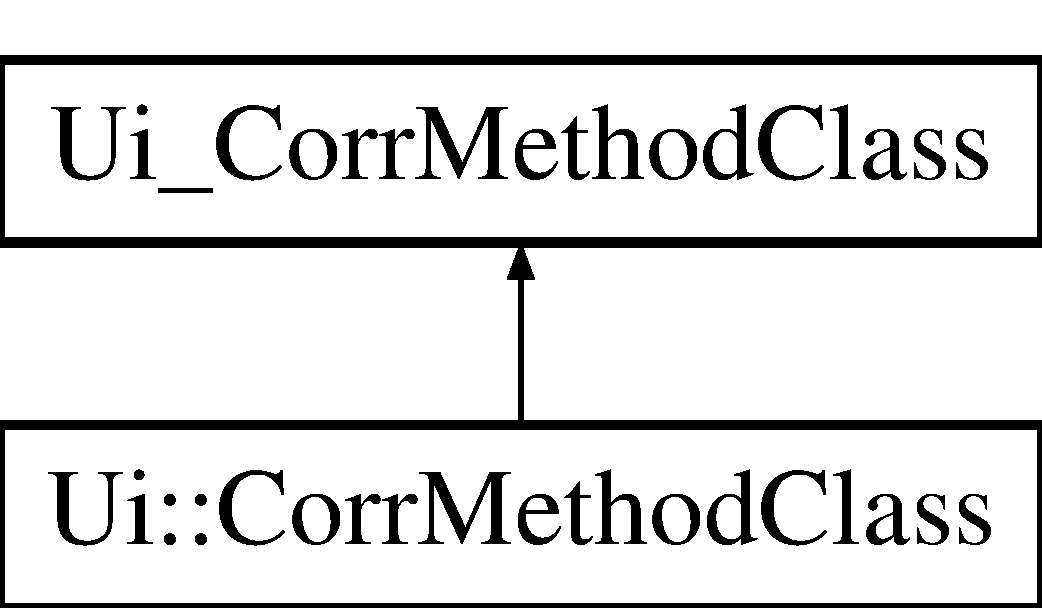
\includegraphics[height=2cm]{classUi_1_1CorrMethodClass}
\end{center}
\end{figure}


\subsection{Detailed Description}


Definition at line 132 of file ui\_\-corrmethod.h.

The documentation for this class was generated from the following file:\begin{DoxyCompactItemize}
\item 
ui\_\-corrmethod.h\end{DoxyCompactItemize}

\hypertarget{classImgLabel}{
\section{ImgLabel Class Reference}
\label{classImgLabel}\index{ImgLabel@{ImgLabel}}
}


\subsection{Detailed Description}


Definition at line 19 of file imgLabel.h.

The documentation for this class was generated from the following file:\begin{DoxyCompactItemize}
\item 
src/imgLabel.h\end{DoxyCompactItemize}

\hypertarget{classImgLabel}{
\section{ImgLabel Class Reference}
\label{classImgLabel}\index{ImgLabel@{ImgLabel}}
}


\subsection{Detailed Description}


Definition at line 19 of file imgLabel.h.

The documentation for this class was generated from the following file:\begin{DoxyCompactItemize}
\item 
src/imgLabel.h\end{DoxyCompactItemize}

\hypertarget{classQcorr}{
\section{Qcorr Class Reference}
\label{classQcorr}\index{Qcorr@{Qcorr}}
}


A Digital Image Correlation Program (Template Matcher) implemented in QT4.  


{\ttfamily \#include $<$src/qcorr.h$>$}Inheritance diagram for Qcorr::\begin{figure}[H]
\begin{center}
\leavevmode
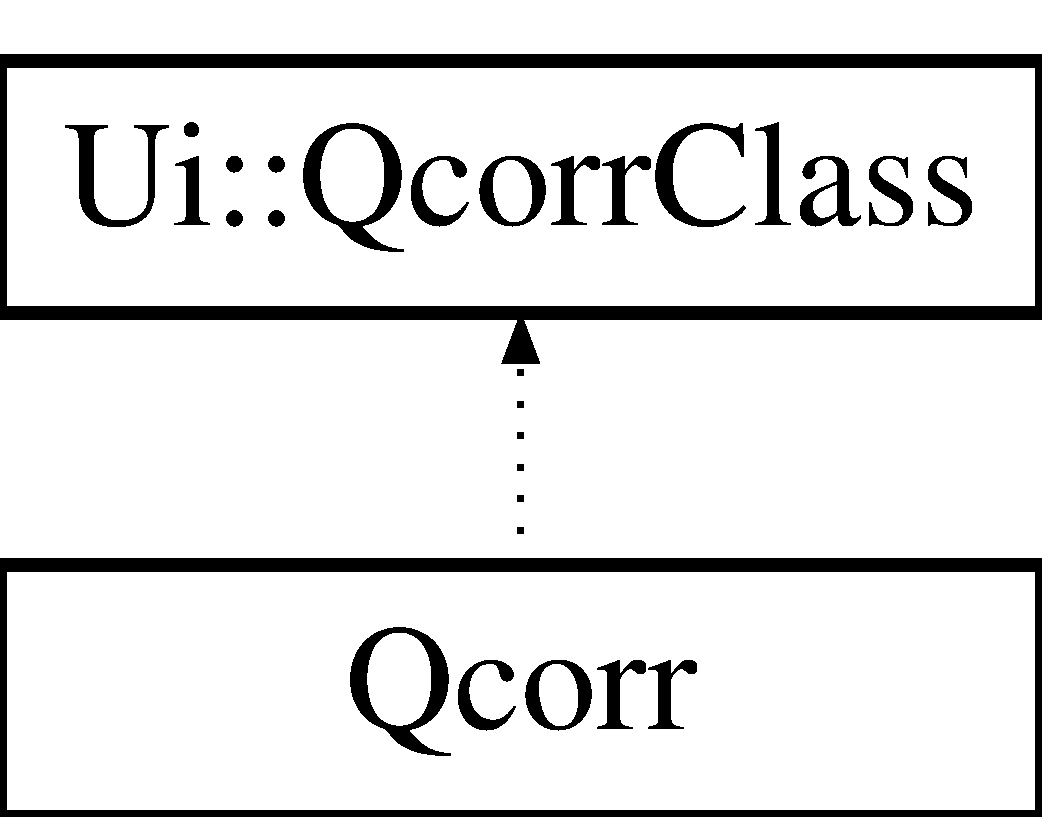
\includegraphics[height=2cm]{classQcorr}
\end{center}
\end{figure}
\subsection*{Public Member Functions}
\begin{DoxyCompactItemize}
\item 
\hypertarget{classQcorr_a3b5d03aed21bfd00497ff265d898e45b}{
{\bfseries Qcorr} (QWidget $\ast$parent=0)}
\label{classQcorr_a3b5d03aed21bfd00497ff265d898e45b}

\end{DoxyCompactItemize}
\subsection*{Private Slots}
\begin{DoxyCompactItemize}
\item 
\hypertarget{classQcorr_adb32e7bfe6afb84f306a9eb5bcd9b322}{
void {\bfseries browseLeftImage} ()}
\label{classQcorr_adb32e7bfe6afb84f306a9eb5bcd9b322}

\item 
\hypertarget{classQcorr_a60583105115d8d14c5fa2a959dc0f285}{
void {\bfseries browseRightImage} ()}
\label{classQcorr_a60583105115d8d14c5fa2a959dc0f285}

\item 
\hypertarget{classQcorr_aa038b382c62558414f6d4592cd039158}{
void {\bfseries viewCorrMap} ()}
\label{classQcorr_aa038b382c62558414f6d4592cd039158}

\item 
\hypertarget{classQcorr_ace91b9d83b34887735737323bac5431e}{
void {\bfseries correlate} ()}
\label{classQcorr_ace91b9d83b34887735737323bac5431e}

\end{DoxyCompactItemize}
\subsection*{Private Member Functions}
\begin{DoxyCompactItemize}
\item 
\hypertarget{classQcorr_a925b0715143a0afa981851547f8b9256}{
void {\bfseries displayImage} (QImage $\ast$image, QLabel $\ast$label)}
\label{classQcorr_a925b0715143a0afa981851547f8b9256}

\item 
\hypertarget{classQcorr_afddb022a6024a32be3b47016308d6c50}{
void {\bfseries displayImageLabel} (QImage $\ast$image, \hyperlink{classImgLabel}{ImgLabel} $\ast$label)}
\label{classQcorr_afddb022a6024a32be3b47016308d6c50}

\item 
\hypertarget{classQcorr_a54af608880477563fa8ebcb0d066b447}{
void {\bfseries createActions} ()}
\label{classQcorr_a54af608880477563fa8ebcb0d066b447}

\item 
\hypertarget{classQcorr_a17beb7cf946cdd82f587e3b4e5ee7f19}{
void {\bfseries setImageLabels} ()}
\label{classQcorr_a17beb7cf946cdd82f587e3b4e5ee7f19}

\item 
float \hyperlink{classQcorr_aa867dbbe79fe720631216eec154a12e2}{findCorrelation} (const unsigned char $\ast$imgTarget, const int nWI, const int nHI, const int nDepthI, const unsigned char $\ast$imgTemplate, const int nWT, const int nHT, const int nDepthT, int \&rnDx, int \&rnDy, int nMethod, bool bMultires)
\begin{DoxyCompactList}\small\item\em Cross-\/correlation of target image with template image. \item\end{DoxyCompactList}\item 
float $\ast$ \hyperlink{classQcorr_ad1b26ace597c0c4a0f64a0bd9576d4fc}{convertToGrayScaleFloat} (const unsigned char $\ast$pchImgOriginalBits, int nSize, int nDepth)
\begin{DoxyCompactList}\small\item\em Cast images to an 8-\/bit gray-\/scale channel of type float. \item\end{DoxyCompactList}\item 
\hypertarget{classQcorr_a87229fc918fa4011e96fbadb325fd52e}{
bool {\bfseries fileDumpQImage} (const QString \&fileName)}
\label{classQcorr_a87229fc918fa4011e96fbadb325fd52e}

\end{DoxyCompactItemize}
\subsection*{Private Attributes}
\begin{DoxyCompactItemize}
\item 
\hypertarget{classQcorr_a49ad0fbdccdce18062eb17bb3ead20ce}{
int {\bfseries m\_\-nXoffset}}
\label{classQcorr_a49ad0fbdccdce18062eb17bb3ead20ce}

\item 
\hypertarget{classQcorr_a882514fa3899bfa373660f643ee85cf7}{
int {\bfseries m\_\-nYoffset}}
\label{classQcorr_a882514fa3899bfa373660f643ee85cf7}

\item 
\hypertarget{classQcorr_a6509fcbf4cd8925aa109cc53e638b69a}{
\hyperlink{classCorrMethod}{CorrMethod} $\ast$ {\bfseries m\_\-corrMethodDialog}}
\label{classQcorr_a6509fcbf4cd8925aa109cc53e638b69a}

\item 
\hypertarget{classQcorr_a3430716ddbe203f677095c163da87f86}{
QString {\bfseries initialName}}
\label{classQcorr_a3430716ddbe203f677095c163da87f86}

\item 
\hypertarget{classQcorr_ae8bdd4be8a0c3023be34a1301b28c913}{
QImage $\ast$ {\bfseries m\_\-leftImage}}
\label{classQcorr_ae8bdd4be8a0c3023be34a1301b28c913}

\item 
\hypertarget{classQcorr_aae1695d731f191c694186e00b96f469e}{
QImage $\ast$ {\bfseries m\_\-rightImage}}
\label{classQcorr_aae1695d731f191c694186e00b96f469e}

\item 
\hypertarget{classQcorr_a5594d939890f10991da0009e4c32bea3}{
QImage $\ast$ {\bfseries m\_\-templateImage}}
\label{classQcorr_a5594d939890f10991da0009e4c32bea3}

\item 
\hypertarget{classQcorr_ac7dc2785613864bea2d8bb0b5f009f36}{
QImage $\ast$ {\bfseries m\_\-corrMapImage}}
\label{classQcorr_ac7dc2785613864bea2d8bb0b5f009f36}

\item 
\hypertarget{classQcorr_acadb3032fbf41f8f1b27067c2784efef}{
\hyperlink{classImgLabel}{ImgLabel} $\ast$ {\bfseries m\_\-leftImage\_\-label}}
\label{classQcorr_acadb3032fbf41f8f1b27067c2784efef}

\item 
\hypertarget{classQcorr_a8d1e1ab866a811003c435c45de1e958e}{
\hyperlink{classTargetImgLabel}{TargetImgLabel} $\ast$ {\bfseries m\_\-targetImage\_\-label}}
\label{classQcorr_a8d1e1ab866a811003c435c45de1e958e}

\item 
\hypertarget{classQcorr_a1bf4a70aa6c4e171f2e0613109bb57e9}{
QLabel $\ast$ {\bfseries m\_\-status\_\-label}}
\label{classQcorr_a1bf4a70aa6c4e171f2e0613109bb57e9}

\item 
\hypertarget{classQcorr_a8a7f00160ae46441cef038149cf28bdc}{
QPoint \hyperlink{classQcorr_a8a7f00160ae46441cef038149cf28bdc}{m\_\-matchingPoint}}
\label{classQcorr_a8a7f00160ae46441cef038149cf28bdc}

\begin{DoxyCompactList}\small\item\em upper-\/left corner point where the correlation match was found \item\end{DoxyCompactList}\item 
\hypertarget{classQcorr_abc48bdd2110cfdaf7b98dde1cdf42f18}{
QSize {\bfseries m\_\-templateSize}}
\label{classQcorr_abc48bdd2110cfdaf7b98dde1cdf42f18}

\end{DoxyCompactItemize}
\subsection*{Friends}
\begin{DoxyCompactItemize}
\item 
\hypertarget{classQcorr_a5b4b2caf4c596b601dd096785e4a32b9}{
class \hyperlink{classQcorr_a5b4b2caf4c596b601dd096785e4a32b9}{ImgLabel}}
\label{classQcorr_a5b4b2caf4c596b601dd096785e4a32b9}

\end{DoxyCompactItemize}


\subsection{Detailed Description}
A Digital Image Correlation Program (Template Matcher) implemented in QT4. This class combines all other sub-\/classed QWidgets implemented throughout the program. The main correlation (template matching) functionality is implemented in this class through the procedure \hyperlink{classQcorr_ad1b26ace597c0c4a0f64a0bd9576d4fc}{convertToGrayScaleFloat()}

\begin{DoxyNote}{Note}

\end{DoxyNote}
Correlation is performed on gray-\/scale (1 channel image) that are computed in this procedure through the \hyperlink{classQcorr_ad1b26ace597c0c4a0f64a0bd9576d4fc}{convertToGrayScaleFloat()} function.

\begin{DoxyParagraph}{Compile-\/time dependencies}

\end{DoxyParagraph}

\begin{DoxyItemize}
\item The QT4 Framework
\end{DoxyItemize}

\begin{Desc}
\item[\hyperlink{bug__bug000001}{Bug}]
\begin{DoxyItemize}
\item Perhaps a few, but not noticed so far.
\end{DoxyItemize}\end{Desc}
\begin{Desc}
\item[\hyperlink{todo__todo000001}{Todo}]
\begin{DoxyItemize}
\item Add Stereo functionality to obtain disparity maps
\end{DoxyItemize}\end{Desc}
\begin{DoxyAuthor}{Author}
Carlos Jaramillo 

Joel Gonzalez 
\end{DoxyAuthor}


Definition at line 48 of file qcorr.h.

\subsection{Member Function Documentation}
\hypertarget{classQcorr_ad1b26ace597c0c4a0f64a0bd9576d4fc}{
\index{Qcorr@{Qcorr}!convertToGrayScaleFloat@{convertToGrayScaleFloat}}
\index{convertToGrayScaleFloat@{convertToGrayScaleFloat}!Qcorr@{Qcorr}}
\subsubsection[{convertToGrayScaleFloat}]{\setlength{\rightskip}{0pt plus 5cm}float $\ast$ Qcorr::convertToGrayScaleFloat (const unsigned char $\ast$ {\em pchImgOriginalBits}, \/  int {\em nSize}, \/  int {\em nDepth})\hspace{0.3cm}{\ttfamily  \mbox{[}private\mbox{]}}}}
\label{classQcorr_ad1b26ace597c0c4a0f64a0bd9576d4fc}


Cast images to an 8-\/bit gray-\/scale channel of type float. 
\begin{DoxyParams}{Parameters}
\item[{\em pchImgOriginalBits}]Buffer of unsigned characters as the source image \item[{\em nSize}]Number of pixels in the source image \item[{\em nDepth}]Pixel depth of the source image \end{DoxyParams}
\begin{DoxyReturn}{Returns}
the correlation number computed by method (directly). Additionally, the (dx,dy) offset of the template for which there exists a best match. 
\end{DoxyReturn}


Definition at line 876 of file qcorr.cpp.

Referenced by findCorrelation().\hypertarget{classQcorr_aa867dbbe79fe720631216eec154a12e2}{
\index{Qcorr@{Qcorr}!findCorrelation@{findCorrelation}}
\index{findCorrelation@{findCorrelation}!Qcorr@{Qcorr}}
\subsubsection[{findCorrelation}]{\setlength{\rightskip}{0pt plus 5cm}float Qcorr::findCorrelation (const unsigned char $\ast$ {\em imgTarget}, \/  const int {\em nWI}, \/  const int {\em nHI}, \/  const int {\em nDepthI}, \/  const unsigned char $\ast$ {\em imgTemplate}, \/  const int {\em nWT}, \/  const int {\em nHT}, \/  const int {\em nDepthT}, \/  int \& {\em rnDx}, \/  int \& {\em rnDy}, \/  int {\em nMethod}, \/  bool {\em bMultires})\hspace{0.3cm}{\ttfamily  \mbox{[}private\mbox{]}}}}
\label{classQcorr_aa867dbbe79fe720631216eec154a12e2}


Cross-\/correlation of target image with template image. \begin{DoxyNote}{Note}
Correlation is performed on gray-\/scale (1 channel image) that are computed in this procedure through the \hyperlink{classQcorr_ad1b26ace597c0c4a0f64a0bd9576d4fc}{convertToGrayScaleFloat()} function. 
\end{DoxyNote}

\begin{DoxyParams}{Parameters}
\item[{\em imgTarget}]Buffer of unsigned characters containing the target image where correlation match is to be found \item[{\em nWI}]Width of target image \item[{\em nHI}]Height of target image \item[{\em nDepthI}]Pixel depth of target image \item[{\em imgTemplate}]Buffer of unsigned characters containing the template image \item[{\em nWT}]Width of target image \item[{\em nHT}]Height of target image \item[{\em nDepthT}]Pixel depth of target image \item[{\em rnDx}]X position where the highest level of correlation match is found (top-\/left corner of the match) \item[{\em rnDy}]Y position where the highest level of correlation match is found (top-\/left corner of the match) \item[{\em method}]Determines the selected method to be used in the correlation process. The method is a globally defined enumeration. The available methods are:
\begin{DoxyItemize}
\item CROSS\_\-CORR (cross correlation): \[ C(u,v) = \frac {\sum{\left\{T(x,y) * I(x-u,y-v)\right\}}} {\sqrt{ \sum{I(x-u,y-v)^2}}} \]
\item SUM\_\-SQ\_\-DIFF (sum of squared differences): \[ C(u,v) = \frac {\sum{\left\{T(x,y)-I(x-u,y-v)\right\}^2}} {\sqrt{\sum{I(x-u,y-v)^2}}} \]
\item CORR\_\-COEFF (correlation coefficient): \[ C(u,v) = \frac {\sum{\left\{(T(x,y)-T_{avg}) * (I(x-u,y-v)-I_{avg})\right\}}} {\sqrt{\sum{(T(x,y)-T_{avg})^2} * \sum{(I(x-u,y-v)-I_{avg})^2}}} \] 
\end{DoxyItemize}\item[{\em multires}]Determines if multiresolution correlation should be applied, by making use of image pyramids. With multiresoltion, the correlation can be determined faster than direct correlation. \end{DoxyParams}
\begin{DoxyReturn}{Returns}
a float array resulting from the conversion of the source image into an 8-\/bit gray-\/scale image. 
\end{DoxyReturn}


Definition at line 262 of file qcorr.cpp.

References convertToGrayScaleFloat().

The documentation for this class was generated from the following files:\begin{DoxyCompactItemize}
\item 
src/qcorr.h\item 
src/qcorr.cpp\end{DoxyCompactItemize}

\hypertarget{classQcorr}{
\section{Qcorr Class Reference}
\label{classQcorr}\index{Qcorr@{Qcorr}}
}


A Digital Image Correlation Program (Template Matcher) implemented in QT4.  


{\ttfamily \#include $<$src/qcorr.h$>$}Inheritance diagram for Qcorr::\begin{figure}[H]
\begin{center}
\leavevmode
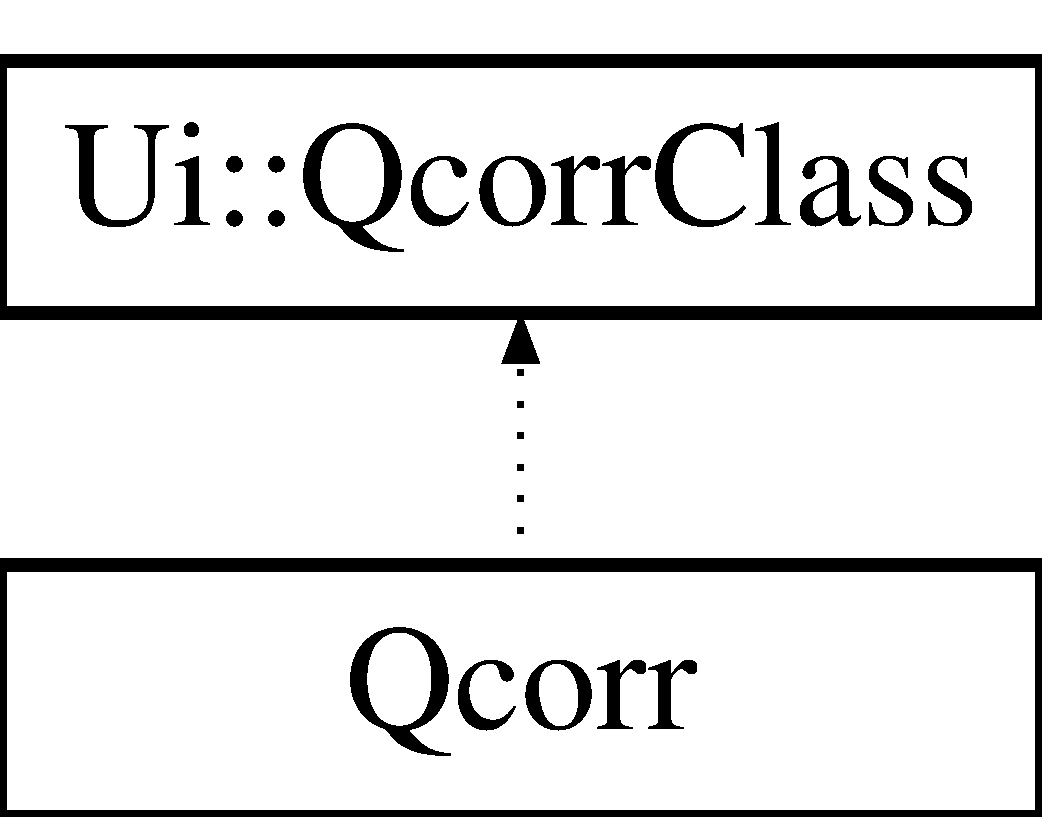
\includegraphics[height=2cm]{classQcorr}
\end{center}
\end{figure}
\subsection*{Public Member Functions}
\begin{DoxyCompactItemize}
\item 
\hypertarget{classQcorr_a3b5d03aed21bfd00497ff265d898e45b}{
{\bfseries Qcorr} (QWidget $\ast$parent=0)}
\label{classQcorr_a3b5d03aed21bfd00497ff265d898e45b}

\end{DoxyCompactItemize}
\subsection*{Private Slots}
\begin{DoxyCompactItemize}
\item 
\hypertarget{classQcorr_adb32e7bfe6afb84f306a9eb5bcd9b322}{
void {\bfseries browseLeftImage} ()}
\label{classQcorr_adb32e7bfe6afb84f306a9eb5bcd9b322}

\item 
\hypertarget{classQcorr_a60583105115d8d14c5fa2a959dc0f285}{
void {\bfseries browseRightImage} ()}
\label{classQcorr_a60583105115d8d14c5fa2a959dc0f285}

\item 
\hypertarget{classQcorr_aa038b382c62558414f6d4592cd039158}{
void {\bfseries viewCorrMap} ()}
\label{classQcorr_aa038b382c62558414f6d4592cd039158}

\item 
\hypertarget{classQcorr_ace91b9d83b34887735737323bac5431e}{
void {\bfseries correlate} ()}
\label{classQcorr_ace91b9d83b34887735737323bac5431e}

\end{DoxyCompactItemize}
\subsection*{Private Member Functions}
\begin{DoxyCompactItemize}
\item 
\hypertarget{classQcorr_a925b0715143a0afa981851547f8b9256}{
void {\bfseries displayImage} (QImage $\ast$image, QLabel $\ast$label)}
\label{classQcorr_a925b0715143a0afa981851547f8b9256}

\item 
\hypertarget{classQcorr_afddb022a6024a32be3b47016308d6c50}{
void {\bfseries displayImageLabel} (QImage $\ast$image, \hyperlink{classImgLabel}{ImgLabel} $\ast$label)}
\label{classQcorr_afddb022a6024a32be3b47016308d6c50}

\item 
\hypertarget{classQcorr_a54af608880477563fa8ebcb0d066b447}{
void {\bfseries createActions} ()}
\label{classQcorr_a54af608880477563fa8ebcb0d066b447}

\item 
\hypertarget{classQcorr_a17beb7cf946cdd82f587e3b4e5ee7f19}{
void {\bfseries setImageLabels} ()}
\label{classQcorr_a17beb7cf946cdd82f587e3b4e5ee7f19}

\item 
float \hyperlink{classQcorr_aa867dbbe79fe720631216eec154a12e2}{findCorrelation} (const unsigned char $\ast$imgTarget, const int nWI, const int nHI, const int nDepthI, const unsigned char $\ast$imgTemplate, const int nWT, const int nHT, const int nDepthT, int \&rnDx, int \&rnDy, int nMethod, bool bMultires)
\begin{DoxyCompactList}\small\item\em Cross-\/correlation of target image with template image. \item\end{DoxyCompactList}\item 
float $\ast$ \hyperlink{classQcorr_ad1b26ace597c0c4a0f64a0bd9576d4fc}{convertToGrayScaleFloat} (const unsigned char $\ast$pchImgOriginalBits, int nSize, int nDepth)
\begin{DoxyCompactList}\small\item\em Cast images to an 8-\/bit gray-\/scale channel of type float. \item\end{DoxyCompactList}\item 
\hypertarget{classQcorr_a87229fc918fa4011e96fbadb325fd52e}{
bool {\bfseries fileDumpQImage} (const QString \&fileName)}
\label{classQcorr_a87229fc918fa4011e96fbadb325fd52e}

\end{DoxyCompactItemize}
\subsection*{Private Attributes}
\begin{DoxyCompactItemize}
\item 
\hypertarget{classQcorr_a49ad0fbdccdce18062eb17bb3ead20ce}{
int {\bfseries m\_\-nXoffset}}
\label{classQcorr_a49ad0fbdccdce18062eb17bb3ead20ce}

\item 
\hypertarget{classQcorr_a882514fa3899bfa373660f643ee85cf7}{
int {\bfseries m\_\-nYoffset}}
\label{classQcorr_a882514fa3899bfa373660f643ee85cf7}

\item 
\hypertarget{classQcorr_a6509fcbf4cd8925aa109cc53e638b69a}{
\hyperlink{classCorrMethod}{CorrMethod} $\ast$ {\bfseries m\_\-corrMethodDialog}}
\label{classQcorr_a6509fcbf4cd8925aa109cc53e638b69a}

\item 
\hypertarget{classQcorr_a3430716ddbe203f677095c163da87f86}{
QString {\bfseries initialName}}
\label{classQcorr_a3430716ddbe203f677095c163da87f86}

\item 
\hypertarget{classQcorr_ae8bdd4be8a0c3023be34a1301b28c913}{
QImage $\ast$ {\bfseries m\_\-leftImage}}
\label{classQcorr_ae8bdd4be8a0c3023be34a1301b28c913}

\item 
\hypertarget{classQcorr_aae1695d731f191c694186e00b96f469e}{
QImage $\ast$ {\bfseries m\_\-rightImage}}
\label{classQcorr_aae1695d731f191c694186e00b96f469e}

\item 
\hypertarget{classQcorr_a5594d939890f10991da0009e4c32bea3}{
QImage $\ast$ {\bfseries m\_\-templateImage}}
\label{classQcorr_a5594d939890f10991da0009e4c32bea3}

\item 
\hypertarget{classQcorr_ac7dc2785613864bea2d8bb0b5f009f36}{
QImage $\ast$ {\bfseries m\_\-corrMapImage}}
\label{classQcorr_ac7dc2785613864bea2d8bb0b5f009f36}

\item 
\hypertarget{classQcorr_acadb3032fbf41f8f1b27067c2784efef}{
\hyperlink{classImgLabel}{ImgLabel} $\ast$ {\bfseries m\_\-leftImage\_\-label}}
\label{classQcorr_acadb3032fbf41f8f1b27067c2784efef}

\item 
\hypertarget{classQcorr_a8d1e1ab866a811003c435c45de1e958e}{
\hyperlink{classTargetImgLabel}{TargetImgLabel} $\ast$ {\bfseries m\_\-targetImage\_\-label}}
\label{classQcorr_a8d1e1ab866a811003c435c45de1e958e}

\item 
\hypertarget{classQcorr_a1bf4a70aa6c4e171f2e0613109bb57e9}{
QLabel $\ast$ {\bfseries m\_\-status\_\-label}}
\label{classQcorr_a1bf4a70aa6c4e171f2e0613109bb57e9}

\item 
\hypertarget{classQcorr_a8a7f00160ae46441cef038149cf28bdc}{
QPoint \hyperlink{classQcorr_a8a7f00160ae46441cef038149cf28bdc}{m\_\-matchingPoint}}
\label{classQcorr_a8a7f00160ae46441cef038149cf28bdc}

\begin{DoxyCompactList}\small\item\em upper-\/left corner point where the correlation match was found \item\end{DoxyCompactList}\item 
\hypertarget{classQcorr_abc48bdd2110cfdaf7b98dde1cdf42f18}{
QSize {\bfseries m\_\-templateSize}}
\label{classQcorr_abc48bdd2110cfdaf7b98dde1cdf42f18}

\end{DoxyCompactItemize}
\subsection*{Friends}
\begin{DoxyCompactItemize}
\item 
\hypertarget{classQcorr_a5b4b2caf4c596b601dd096785e4a32b9}{
class \hyperlink{classQcorr_a5b4b2caf4c596b601dd096785e4a32b9}{ImgLabel}}
\label{classQcorr_a5b4b2caf4c596b601dd096785e4a32b9}

\end{DoxyCompactItemize}


\subsection{Detailed Description}
A Digital Image Correlation Program (Template Matcher) implemented in QT4. This class combines all other sub-\/classed QWidgets implemented throughout the program. The main correlation (template matching) functionality is implemented in this class through the procedure \hyperlink{classQcorr_ad1b26ace597c0c4a0f64a0bd9576d4fc}{convertToGrayScaleFloat()}

\begin{DoxyNote}{Note}

\end{DoxyNote}
Correlation is performed on gray-\/scale (1 channel image) that are computed in this procedure through the \hyperlink{classQcorr_ad1b26ace597c0c4a0f64a0bd9576d4fc}{convertToGrayScaleFloat()} function.

\begin{DoxyParagraph}{Compile-\/time dependencies}

\end{DoxyParagraph}

\begin{DoxyItemize}
\item The QT4 Framework
\end{DoxyItemize}

\begin{Desc}
\item[\hyperlink{bug__bug000001}{Bug}]
\begin{DoxyItemize}
\item Perhaps a few, but not noticed so far.
\end{DoxyItemize}\end{Desc}
\begin{Desc}
\item[\hyperlink{todo__todo000001}{Todo}]
\begin{DoxyItemize}
\item Add Stereo functionality to obtain disparity maps
\end{DoxyItemize}\end{Desc}
\begin{DoxyAuthor}{Author}
Carlos Jaramillo 

Joel Gonzalez 
\end{DoxyAuthor}


Definition at line 48 of file qcorr.h.

\subsection{Member Function Documentation}
\hypertarget{classQcorr_ad1b26ace597c0c4a0f64a0bd9576d4fc}{
\index{Qcorr@{Qcorr}!convertToGrayScaleFloat@{convertToGrayScaleFloat}}
\index{convertToGrayScaleFloat@{convertToGrayScaleFloat}!Qcorr@{Qcorr}}
\subsubsection[{convertToGrayScaleFloat}]{\setlength{\rightskip}{0pt plus 5cm}float $\ast$ Qcorr::convertToGrayScaleFloat (const unsigned char $\ast$ {\em pchImgOriginalBits}, \/  int {\em nSize}, \/  int {\em nDepth})\hspace{0.3cm}{\ttfamily  \mbox{[}private\mbox{]}}}}
\label{classQcorr_ad1b26ace597c0c4a0f64a0bd9576d4fc}


Cast images to an 8-\/bit gray-\/scale channel of type float. 
\begin{DoxyParams}{Parameters}
\item[{\em pchImgOriginalBits}]Buffer of unsigned characters as the source image \item[{\em nSize}]Number of pixels in the source image \item[{\em nDepth}]Pixel depth of the source image \end{DoxyParams}
\begin{DoxyReturn}{Returns}
the correlation number computed by method (directly). Additionally, the (dx,dy) offset of the template for which there exists a best match. 
\end{DoxyReturn}


Definition at line 876 of file qcorr.cpp.

Referenced by findCorrelation().\hypertarget{classQcorr_aa867dbbe79fe720631216eec154a12e2}{
\index{Qcorr@{Qcorr}!findCorrelation@{findCorrelation}}
\index{findCorrelation@{findCorrelation}!Qcorr@{Qcorr}}
\subsubsection[{findCorrelation}]{\setlength{\rightskip}{0pt plus 5cm}float Qcorr::findCorrelation (const unsigned char $\ast$ {\em imgTarget}, \/  const int {\em nWI}, \/  const int {\em nHI}, \/  const int {\em nDepthI}, \/  const unsigned char $\ast$ {\em imgTemplate}, \/  const int {\em nWT}, \/  const int {\em nHT}, \/  const int {\em nDepthT}, \/  int \& {\em rnDx}, \/  int \& {\em rnDy}, \/  int {\em nMethod}, \/  bool {\em bMultires})\hspace{0.3cm}{\ttfamily  \mbox{[}private\mbox{]}}}}
\label{classQcorr_aa867dbbe79fe720631216eec154a12e2}


Cross-\/correlation of target image with template image. \begin{DoxyNote}{Note}
Correlation is performed on gray-\/scale (1 channel image) that are computed in this procedure through the \hyperlink{classQcorr_ad1b26ace597c0c4a0f64a0bd9576d4fc}{convertToGrayScaleFloat()} function. 
\end{DoxyNote}

\begin{DoxyParams}{Parameters}
\item[{\em imgTarget}]Buffer of unsigned characters containing the target image where correlation match is to be found \item[{\em nWI}]Width of target image \item[{\em nHI}]Height of target image \item[{\em nDepthI}]Pixel depth of target image \item[{\em imgTemplate}]Buffer of unsigned characters containing the template image \item[{\em nWT}]Width of target image \item[{\em nHT}]Height of target image \item[{\em nDepthT}]Pixel depth of target image \item[{\em rnDx}]X position where the highest level of correlation match is found (top-\/left corner of the match) \item[{\em rnDy}]Y position where the highest level of correlation match is found (top-\/left corner of the match) \item[{\em method}]Determines the selected method to be used in the correlation process. The method is a globally defined enumeration. The available methods are:
\begin{DoxyItemize}
\item CROSS\_\-CORR (cross correlation): \[ C(u,v) = \frac {\sum{\left\{T(x,y) * I(x-u,y-v)\right\}}} {\sqrt{ \sum{I(x-u,y-v)^2}}} \]
\item SUM\_\-SQ\_\-DIFF (sum of squared differences): \[ C(u,v) = \frac {\sum{\left\{T(x,y)-I(x-u,y-v)\right\}^2}} {\sqrt{\sum{I(x-u,y-v)^2}}} \]
\item CORR\_\-COEFF (correlation coefficient): \[ C(u,v) = \frac {\sum{\left\{(T(x,y)-T_{avg}) * (I(x-u,y-v)-I_{avg})\right\}}} {\sqrt{\sum{(T(x,y)-T_{avg})^2} * \sum{(I(x-u,y-v)-I_{avg})^2}}} \] 
\end{DoxyItemize}\item[{\em multires}]Determines if multiresolution correlation should be applied, by making use of image pyramids. With multiresoltion, the correlation can be determined faster than direct correlation. \end{DoxyParams}
\begin{DoxyReturn}{Returns}
a float array resulting from the conversion of the source image into an 8-\/bit gray-\/scale image. 
\end{DoxyReturn}


Definition at line 262 of file qcorr.cpp.

References convertToGrayScaleFloat().

The documentation for this class was generated from the following files:\begin{DoxyCompactItemize}
\item 
src/qcorr.h\item 
src/qcorr.cpp\end{DoxyCompactItemize}

\hypertarget{classUi_1_1QcorrClass}{
\section{Ui::QcorrClass Class Reference}
\label{classUi_1_1QcorrClass}\index{Ui::QcorrClass@{Ui::QcorrClass}}
}
Inheritance diagram for Ui::QcorrClass::\begin{figure}[H]
\begin{center}
\leavevmode
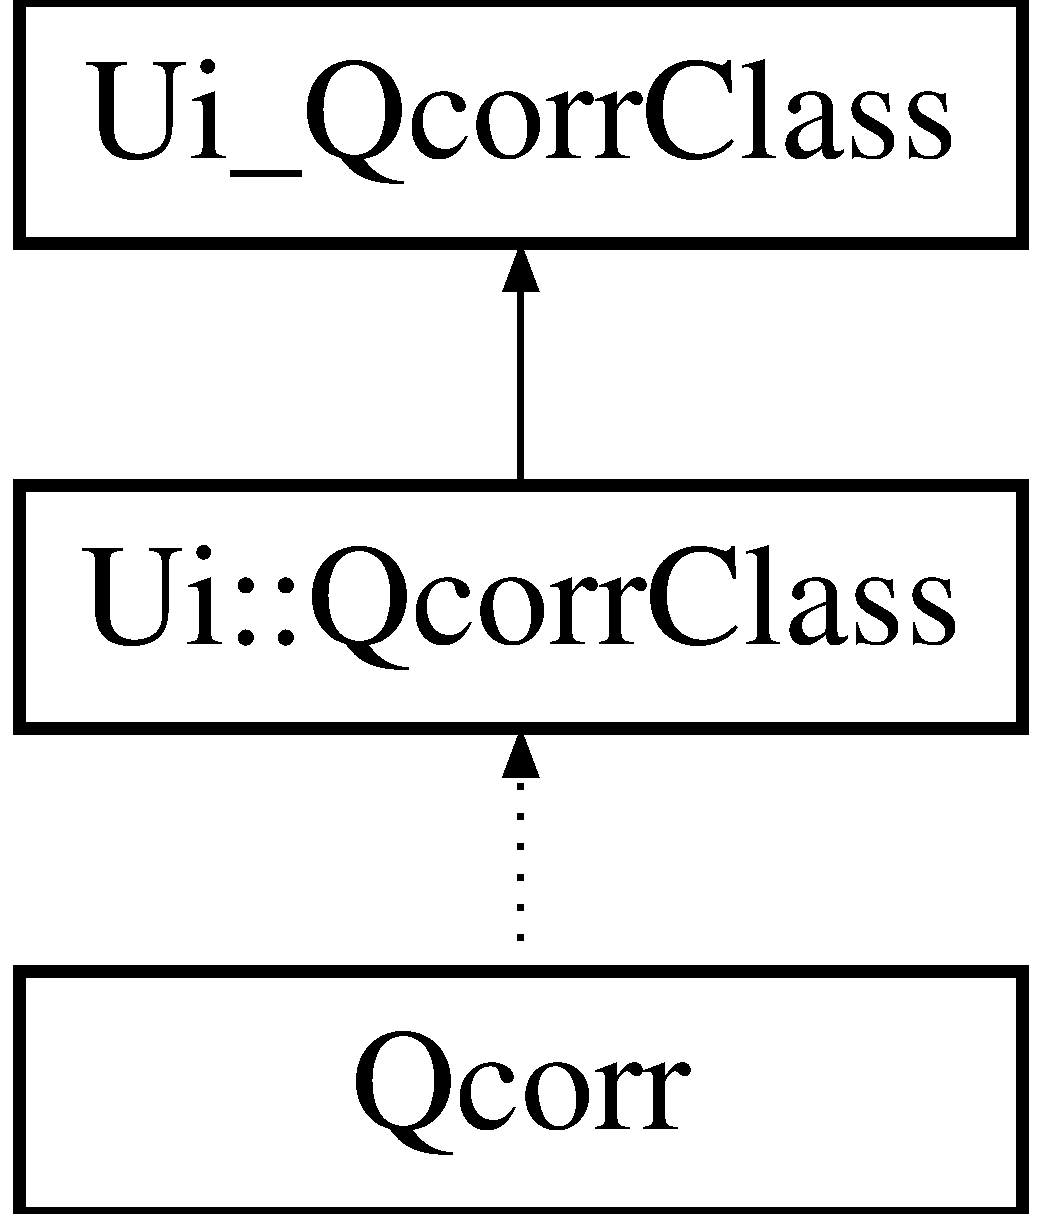
\includegraphics[height=3cm]{classUi_1_1QcorrClass}
\end{center}
\end{figure}


\subsection{Detailed Description}


Definition at line 260 of file ui\_\-qcorr.h.

The documentation for this class was generated from the following file:\begin{DoxyCompactItemize}
\item 
ui\_\-qcorr.h\end{DoxyCompactItemize}

\hypertarget{classTargetImgLabel}{
\section{TargetImgLabel Class Reference}
\label{classTargetImgLabel}\index{TargetImgLabel@{TargetImgLabel}}
}
\subsection*{Public Member Functions}
\begin{DoxyCompactItemize}
\item 
\hypertarget{classTargetImgLabel_acb3dcfa8b9616be0a355c90db81aaba2}{
{\bfseries TargetImgLabel} (QWidget $\ast$parent=0)}
\label{classTargetImgLabel_acb3dcfa8b9616be0a355c90db81aaba2}

\item 
\hypertarget{classTargetImgLabel_a2ec40d8850e3d9cc4d5c9984412c0cfb}{
void {\bfseries setImage} (const QImage \&labelImage)}
\label{classTargetImgLabel_a2ec40d8850e3d9cc4d5c9984412c0cfb}

\item 
\hypertarget{classTargetImgLabel_a719f70b755013a216f2a7b10352dd0fe}{
void {\bfseries overlayImage} (const QImage \&otherImage)}
\label{classTargetImgLabel_a719f70b755013a216f2a7b10352dd0fe}

\item 
\hypertarget{classTargetImgLabel_ab835774d14df1e93cb0fd010d1a2e699}{
void {\bfseries drawEnclosedMatch} (const QPoint originPoint, const QSize rectSize)}
\label{classTargetImgLabel_ab835774d14df1e93cb0fd010d1a2e699}

\item 
\hypertarget{classTargetImgLabel_ad060485d97c7797339243b23f3ea05ef}{
void {\bfseries eraseEnclosedMatch} ()}
\label{classTargetImgLabel_ad060485d97c7797339243b23f3ea05ef}

\end{DoxyCompactItemize}
\subsection*{Protected Member Functions}
\begin{DoxyCompactItemize}
\item 
\hypertarget{classTargetImgLabel_a30f9fc1657bdf5a9459bd78d5a94c65b}{
void {\bfseries paintEvent} (QPaintEvent $\ast$)}
\label{classTargetImgLabel_a30f9fc1657bdf5a9459bd78d5a94c65b}

\end{DoxyCompactItemize}
\subsection*{Private Attributes}
\begin{DoxyCompactItemize}
\item 
\hypertarget{classTargetImgLabel_ae532d541556a3647cff5a83bcf1306c3}{
QImage $\ast$ {\bfseries m\_\-image}}
\label{classTargetImgLabel_ae532d541556a3647cff5a83bcf1306c3}

\item 
\hypertarget{classTargetImgLabel_a94cf2b5841057d54bf3172aa2fef1e83}{
QImage $\ast$ {\bfseries m\_\-overlayImage}}
\label{classTargetImgLabel_a94cf2b5841057d54bf3172aa2fef1e83}

\item 
\hypertarget{classTargetImgLabel_a0ed69ba29f03494cdd3ec22d9df4e15f}{
QPoint {\bfseries m\_\-originPoint}}
\label{classTargetImgLabel_a0ed69ba29f03494cdd3ec22d9df4e15f}

\item 
\hypertarget{classTargetImgLabel_ae9e4109bdd7a8a6b5d0bd59850c6abba}{
QSize {\bfseries m\_\-rectSize}}
\label{classTargetImgLabel_ae9e4109bdd7a8a6b5d0bd59850c6abba}

\item 
\hypertarget{classTargetImgLabel_a34a2b6061eb38412b7f7e88fbf741c2f}{
bool {\bfseries m\_\-bHasCorrResults}}
\label{classTargetImgLabel_a34a2b6061eb38412b7f7e88fbf741c2f}

\item 
\hypertarget{classTargetImgLabel_a3b0b34d9c2f7c4f6c9aea8bc75d91d99}{
bool {\bfseries m\_\-bHasImage}}
\label{classTargetImgLabel_a3b0b34d9c2f7c4f6c9aea8bc75d91d99}

\item 
\hypertarget{classTargetImgLabel_a1c34173d16f00af22f7db9e1bb3e7b30}{
bool {\bfseries m\_\-bHasOverlayImage}}
\label{classTargetImgLabel_a1c34173d16f00af22f7db9e1bb3e7b30}

\end{DoxyCompactItemize}


\subsection{Detailed Description}


Definition at line 17 of file targetImgLabel.h.

The documentation for this class was generated from the following files:\begin{DoxyCompactItemize}
\item 
src/targetImgLabel.h\item 
src/targetImgLabel.cpp\end{DoxyCompactItemize}

\include{classUi__ControlsWindowClass}
\hypertarget{classUi__CorrMethodClass}{
\section{Ui\_\-CorrMethodClass Class Reference}
\label{classUi__CorrMethodClass}\index{Ui\_\-CorrMethodClass@{Ui\_\-CorrMethodClass}}
}
Inheritance diagram for Ui\_\-CorrMethodClass::\begin{figure}[H]
\begin{center}
\leavevmode
\includegraphics[height=2cm]{classUi__CorrMethodClass}
\end{center}
\end{figure}
\subsection*{Public Member Functions}
\begin{DoxyCompactItemize}
\item 
\hypertarget{classUi__CorrMethodClass_a95a6bbb76de087aa2f8f5ea4780a4d09}{
void {\bfseries setupUi} (QDialog $\ast$CorrMethodClass)}
\label{classUi__CorrMethodClass_a95a6bbb76de087aa2f8f5ea4780a4d09}

\item 
\hypertarget{classUi__CorrMethodClass_a4ac1c93be0509c13a248873b5dd7e2fb}{
void {\bfseries retranslateUi} (QDialog $\ast$CorrMethodClass)}
\label{classUi__CorrMethodClass_a4ac1c93be0509c13a248873b5dd7e2fb}

\end{DoxyCompactItemize}
\subsection*{Public Attributes}
\begin{DoxyCompactItemize}
\item 
\hypertarget{classUi__CorrMethodClass_ab3e404afe1c6fafb99e02a2a9315e8d1}{
QFrame $\ast$ {\bfseries dialog\_\-Frame}}
\label{classUi__CorrMethodClass_ab3e404afe1c6fafb99e02a2a9315e8d1}

\item 
\hypertarget{classUi__CorrMethodClass_aab4f631b545d0545adde08190ecab6fa}{
QVBoxLayout $\ast$ {\bfseries verticalLayout}}
\label{classUi__CorrMethodClass_aab4f631b545d0545adde08190ecab6fa}

\item 
\hypertarget{classUi__CorrMethodClass_add008cc6d16e9265345255c6fbc2e0b5}{
QLabel $\ast$ {\bfseries selectMethod\_\-label}}
\label{classUi__CorrMethodClass_add008cc6d16e9265345255c6fbc2e0b5}

\item 
\hypertarget{classUi__CorrMethodClass_a55e61e05e9ff340d17b08f7489e84039}{
QGroupBox $\ast$ {\bfseries methods\_\-groupBox}}
\label{classUi__CorrMethodClass_a55e61e05e9ff340d17b08f7489e84039}

\item 
\hypertarget{classUi__CorrMethodClass_aa260d1145f60cdc7137a93d50f66b2e9}{
QRadioButton $\ast$ {\bfseries method3\_\-radioButton}}
\label{classUi__CorrMethodClass_aa260d1145f60cdc7137a93d50f66b2e9}

\item 
\hypertarget{classUi__CorrMethodClass_acced16b55f7c8baa3c789435616c35c6}{
QRadioButton $\ast$ {\bfseries method2\_\-radioButton}}
\label{classUi__CorrMethodClass_acced16b55f7c8baa3c789435616c35c6}

\item 
\hypertarget{classUi__CorrMethodClass_a091300f07ee518675317d2001e486a42}{
QRadioButton $\ast$ {\bfseries method1\_\-radioButton}}
\label{classUi__CorrMethodClass_a091300f07ee518675317d2001e486a42}

\item 
\hypertarget{classUi__CorrMethodClass_ac4d190aefc50d332cfdc73d7370f4ca2}{
QDialogButtonBox $\ast$ {\bfseries buttonBox}}
\label{classUi__CorrMethodClass_ac4d190aefc50d332cfdc73d7370f4ca2}

\item 
\hypertarget{classUi__CorrMethodClass_ac98460426d7a9f1c1a2763d9e3c0c2ef}{
QSpacerItem $\ast$ {\bfseries verticalSpacer}}
\label{classUi__CorrMethodClass_ac98460426d7a9f1c1a2763d9e3c0c2ef}

\end{DoxyCompactItemize}


\subsection{Detailed Description}


Definition at line 29 of file ui\_\-corrmethod.h.

The documentation for this class was generated from the following file:\begin{DoxyCompactItemize}
\item 
ui\_\-corrmethod.h\end{DoxyCompactItemize}

\hypertarget{classUi__QcorrClass}{
\section{Ui\_\-QcorrClass Class Reference}
\label{classUi__QcorrClass}\index{Ui\_\-QcorrClass@{Ui\_\-QcorrClass}}
}
Inheritance diagram for Ui\_\-QcorrClass::\begin{figure}[H]
\begin{center}
\leavevmode
\includegraphics[height=3cm]{classUi__QcorrClass}
\end{center}
\end{figure}
\subsection*{Public Member Functions}
\begin{DoxyCompactItemize}
\item 
\hypertarget{classUi__QcorrClass_a80aee2ed06f3c4f9b1f516405d888c13}{
void {\bfseries setupUi} (QMainWindow $\ast$QcorrClass)}
\label{classUi__QcorrClass_a80aee2ed06f3c4f9b1f516405d888c13}

\item 
\hypertarget{classUi__QcorrClass_adefed69462e2297254f0d5bce3131e05}{
void {\bfseries retranslateUi} (QMainWindow $\ast$QcorrClass)}
\label{classUi__QcorrClass_adefed69462e2297254f0d5bce3131e05}

\end{DoxyCompactItemize}
\subsection*{Public Attributes}
\begin{DoxyCompactItemize}
\item 
\hypertarget{classUi__QcorrClass_ae725a71d3bb44a43e2d65ce4d1284b85}{
QAction $\ast$ {\bfseries action\_\-Quit}}
\label{classUi__QcorrClass_ae725a71d3bb44a43e2d65ce4d1284b85}

\item 
\hypertarget{classUi__QcorrClass_ae8508d05f75fac71c1f6fdb50fae6d7d}{
QAction $\ast$ {\bfseries action\_\-Correlation\_\-Map}}
\label{classUi__QcorrClass_ae8508d05f75fac71c1f6fdb50fae6d7d}

\item 
\hypertarget{classUi__QcorrClass_a885bdbbc4267078f102878ad126b23bb}{
QWidget $\ast$ {\bfseries centralwidget}}
\label{classUi__QcorrClass_a885bdbbc4267078f102878ad126b23bb}

\item 
\hypertarget{classUi__QcorrClass_acb93f5008511c2654ac8a51c17dc11ef}{
QFrame $\ast$ {\bfseries main\_\-frame}}
\label{classUi__QcorrClass_acb93f5008511c2654ac8a51c17dc11ef}

\item 
\hypertarget{classUi__QcorrClass_afd1d2aad88a740a9f33d9f91370c7ea9}{
QVBoxLayout $\ast$ {\bfseries main\_\-verticalLayout}}
\label{classUi__QcorrClass_afd1d2aad88a740a9f33d9f91370c7ea9}

\item 
\hypertarget{classUi__QcorrClass_ab4e96571e7dd58d9ec798cf6ede3cbe6}{
QSplitter $\ast$ {\bfseries splitter}}
\label{classUi__QcorrClass_ab4e96571e7dd58d9ec798cf6ede3cbe6}

\item 
\hypertarget{classUi__QcorrClass_a81e59812852e521cced5e1f912bffb99}{
QWidget $\ast$ {\bfseries layoutWidget}}
\label{classUi__QcorrClass_a81e59812852e521cced5e1f912bffb99}

\item 
\hypertarget{classUi__QcorrClass_ae7eb5196b5e392a40fa3e3a77f40c3cc}{
QVBoxLayout $\ast$ {\bfseries left\_\-verticalLayout}}
\label{classUi__QcorrClass_ae7eb5196b5e392a40fa3e3a77f40c3cc}

\item 
\hypertarget{classUi__QcorrClass_aaad53db0cbf018c38d75aebbe78959b3}{
QHBoxLayout $\ast$ {\bfseries leftImg\_\-horizontalLayout}}
\label{classUi__QcorrClass_aaad53db0cbf018c38d75aebbe78959b3}

\item 
\hypertarget{classUi__QcorrClass_a12d1c71e330c76e65484418502338a31}{
QLineEdit $\ast$ {\bfseries leftImage\_\-lineEdit}}
\label{classUi__QcorrClass_a12d1c71e330c76e65484418502338a31}

\item 
\hypertarget{classUi__QcorrClass_ae05243dcb19bfd6fd6d1c3257f25338a}{
QPushButton $\ast$ {\bfseries leftBrowse\_\-pushButton}}
\label{classUi__QcorrClass_ae05243dcb19bfd6fd6d1c3257f25338a}

\item 
\hypertarget{classUi__QcorrClass_acb12117880660e7d8fec35de7eee51c6}{
QScrollArea $\ast$ {\bfseries leftImage\_\-scrollArea}}
\label{classUi__QcorrClass_acb12117880660e7d8fec35de7eee51c6}

\item 
\hypertarget{classUi__QcorrClass_aab5ae2e7dc3baefb6ada5e1a758e826f}{
QWidget $\ast$ {\bfseries scrollAreaWidgetContents\_\-3}}
\label{classUi__QcorrClass_aab5ae2e7dc3baefb6ada5e1a758e826f}

\item 
\hypertarget{classUi__QcorrClass_a24caba38fd151a2ab5b577b1425bd07c}{
QWidget $\ast$ {\bfseries layoutWidget1}}
\label{classUi__QcorrClass_a24caba38fd151a2ab5b577b1425bd07c}

\item 
\hypertarget{classUi__QcorrClass_a232c26905d00f6608b8ba97a6546daa0}{
QVBoxLayout $\ast$ {\bfseries right\_\-verticalLayout}}
\label{classUi__QcorrClass_a232c26905d00f6608b8ba97a6546daa0}

\item 
\hypertarget{classUi__QcorrClass_a6885fe1dcc883e2f927c2fb943b206e0}{
QHBoxLayout $\ast$ {\bfseries rightImg\_\-horizontalLayout}}
\label{classUi__QcorrClass_a6885fe1dcc883e2f927c2fb943b206e0}

\item 
\hypertarget{classUi__QcorrClass_a690e51bd7f4916ca89f876f39afee05d}{
QLineEdit $\ast$ {\bfseries rightImage\_\-lineEdit}}
\label{classUi__QcorrClass_a690e51bd7f4916ca89f876f39afee05d}

\item 
\hypertarget{classUi__QcorrClass_a5018f953d94c196394a638212a45fd9d}{
QPushButton $\ast$ {\bfseries rightBrowse\_\-pushButton}}
\label{classUi__QcorrClass_a5018f953d94c196394a638212a45fd9d}

\item 
\hypertarget{classUi__QcorrClass_a227cae34e275c9e0713ee279435f41cc}{
QScrollArea $\ast$ {\bfseries rightImage\_\-scrollArea}}
\label{classUi__QcorrClass_a227cae34e275c9e0713ee279435f41cc}

\item 
\hypertarget{classUi__QcorrClass_abf4b50d1ea6274629f687ac66ce12e80}{
QWidget $\ast$ {\bfseries scrollAreaWidgetContents\_\-2}}
\label{classUi__QcorrClass_abf4b50d1ea6274629f687ac66ce12e80}

\item 
\hypertarget{classUi__QcorrClass_aa4247652a1ed71c6b6704aa3273544bd}{
QHBoxLayout $\ast$ {\bfseries bottom\_\-horizontalLayout}}
\label{classUi__QcorrClass_aa4247652a1ed71c6b6704aa3273544bd}

\item 
\hypertarget{classUi__QcorrClass_a06bd40ad7db57a5438d16e5d5061df42}{
QPushButton $\ast$ {\bfseries corr\_\-pushButton}}
\label{classUi__QcorrClass_a06bd40ad7db57a5438d16e5d5061df42}

\item 
\hypertarget{classUi__QcorrClass_a4ddf4aae819f6b25476a5a3e76c600d7}{
QLabel $\ast$ {\bfseries corrResults\_\-label}}
\label{classUi__QcorrClass_a4ddf4aae819f6b25476a5a3e76c600d7}

\item 
\hypertarget{classUi__QcorrClass_a80762eea1a44f16ceffed065d0459a69}{
QSpacerItem $\ast$ {\bfseries horizontalSpacer}}
\label{classUi__QcorrClass_a80762eea1a44f16ceffed065d0459a69}

\item 
\hypertarget{classUi__QcorrClass_ad032c2f5b8f1aed8decad689900d7017}{
QPushButton $\ast$ {\bfseries quit\_\-pushButton}}
\label{classUi__QcorrClass_ad032c2f5b8f1aed8decad689900d7017}

\item 
\hypertarget{classUi__QcorrClass_a8567acdc882322bab775dd04569433da}{
QMenuBar $\ast$ {\bfseries menubar}}
\label{classUi__QcorrClass_a8567acdc882322bab775dd04569433da}

\item 
\hypertarget{classUi__QcorrClass_a1d52a371f0d1e29cdf70d1be2a85a45e}{
QMenu $\ast$ {\bfseries menu\_\-Menu}}
\label{classUi__QcorrClass_a1d52a371f0d1e29cdf70d1be2a85a45e}

\item 
\hypertarget{classUi__QcorrClass_a8c1dd90b9ea2130b6fe6e8e6553fbf13}{
QMenu $\ast$ {\bfseries menu\_\-View}}
\label{classUi__QcorrClass_a8c1dd90b9ea2130b6fe6e8e6553fbf13}

\item 
\hypertarget{classUi__QcorrClass_ae220680c312c600f015f0413ad6cd2cf}{
QStatusBar $\ast$ {\bfseries statusbar}}
\label{classUi__QcorrClass_ae220680c312c600f015f0413ad6cd2cf}

\end{DoxyCompactItemize}


\subsection{Detailed Description}


Definition at line 35 of file ui\_\-qcorr.h.

The documentation for this class was generated from the following file:\begin{DoxyCompactItemize}
\item 
ui\_\-qcorr.h\end{DoxyCompactItemize}

\printindex
\end{document}
